\documentclass[compress]{beamer}

\usepackage[T1]{fontenc} 
\usepackage{amsmath}
\usepackage{array}
\usepackage{color}
\usepackage{graphicx}
\usepackage[section]{placeins} % force � mettre l'image o� on veut
\usepackage{float} %utiliser H pour forcer � mettre l'image o� on veut
\usepackage{lscape} %utilisation du mode paysage
\usepackage{pslatex}
\usepackage{multimedia}
\usepackage{stmaryrd} % permet d'utiliser \llbracket et \rrbracket : double crochet


\usetheme{Frankfurt}

\setbeamertemplate{footline}{
\leavevmode%
\hbox{\hspace*{-0.06cm}
\begin{beamercolorbox}[wd=.3\paperwidth,ht=2.25ex,dp=1ex,center]{author in head/foot}%
	\usebeamerfont{author in head/foot}\insertshortauthor%~~(\insertshortinstitute)
\end{beamercolorbox}%
\begin{beamercolorbox}[wd=.5\paperwidth,ht=2.25ex,dp=1ex,center]{section in head/foot}%
	\usebeamerfont{section in head/foot}\insertshorttitle
\end{beamercolorbox}%
\begin{beamercolorbox}[wd=.2\paperwidth,ht=2.25ex,dp=1ex,right]{section in head/foot}%
	\usebeamerfont{section in head/foot}\insertshortdate{}\hspace*{2em}
	\insertframenumber{} / \inserttotalframenumber\hspace*{2ex}
\end{beamercolorbox}}%
\vskip0pt%
}

\newcommand\bn{\boldsymbol{\nabla}}
\newcommand\bo{\boldsymbol{\Omega}}
\newcommand\br{\mathbf{r}}
\newcommand\la{\left\langle}
\newcommand\ra{\right\rangle}
\newcommand\bs{\boldsymbol}
\newcommand\red{\textcolor{red}}
\newcommand\ldb{\{\!\{}
\newcommand\rdb{\}\!\}}
\newcommand\llb{\llbracket}
\newcommand\rrb{\rrbracket}

\renewcommand{\(}{\left(}
\renewcommand{\)}{\right)}
\renewcommand{\[}{\left[}
\renewcommand{\]}{\right]}
\beamertemplatetransparentcovered

\title{Charged particles transport}
\author{Bruno Turcksin, Jean Ragusa \& Jim Morel}\institute{Texas A\&M University, Dept. of Nuclear Engineering}
\date{}

\begin{document}

\begin{frame}
\maketitle
\end{frame}
%---------------------------------------------------------------------------------------------
\logo{\includegraphics[height=0.5cm]{logo_Texas.jpg}}
\begin{frame}
\frametitle{Outline}
\tableofcontents[hideallsubsections]
\end{frame}
%---------------------------------------------------------------------------------------------
\section{Introduction}
\subsection{Introduction}
\begin{frame}
\frametitle{Introduction}
\begin{itemize}
\item Radiotherapy is used for cancer treatment.
\item Used Intensity Modulated Radiation Therapy (IMRT).
\item Proton therapy contains the same physics.
\end{itemize}
\begin{figure}[H]
\centering
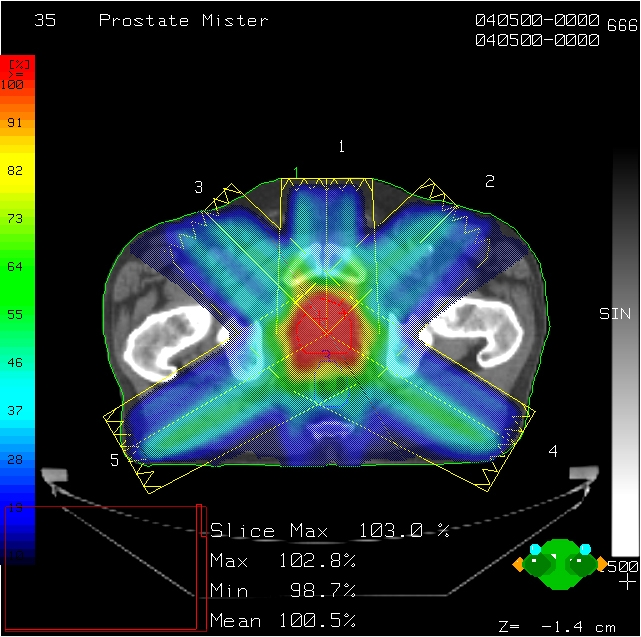
\includegraphics[width=3cm]{IMRT}
\end{figure}
\end{frame}
%---------------------------------------------------------------------------------------------
\section{Boltzmann-CSD}
\subsection{Equations}
\begin{frame}
\frametitle{Equations}
\begin{itemize}
\item Boltzmann equation could be used but electron cross section are very forward $\Rightarrow$ need very high order of Legendre polynomials ($\sim 200$) to approximate the cross section.
\item The Boltzmann-Fokker-Planck equation uses a Boltzmann scattering term for large angle scattering (hard scattering) and the Fokker-Planck terms for small angle scattering (soft scattering).
\end{itemize}
\end{frame}
%---------------------------------------------------------------------------------------------
\begin{frame}
\frametitle{Equations}
Boltzmann-Fokker-Planck equation :
\begin{equation}
\begin{split}
&\bo \cdot \bn \Psi + \Sigma_t \Psi = \int_{-1}^1 d\mu_0 \int_0^{\infty} dE' \Sigma_s(x,\mu_0,E'\rightarrow E) \Psi(x,\mu_0,E') +\\
& \frac{\alpha}{2} \frac{\partial }{\partial \mu} \(1-\mu^2\) \frac{\partial \Psi}{\partial \mu} + \frac{\partial \(S\Psi\)}{\partial E} + Q
\end{split}
\end{equation}
where : 
\begin {itemize}
\item $\alpha$ is the restricted momentum transfer: scattering without loss of energy. 
\item $S$ is the restricted stopping power: loss of energy without scattering (Continuous Slowing Down).
\end{itemize}
\end{frame}
%---------------------------------------------------------------------------------------------
\begin{frame}
\frametitle{Equations}
\begin{itemize}
\item The term $\frac{\alpha}{2} \frac{\partial }{\partial \mu} \(1-\mu^2\) \frac{\partial \Psi}{\partial \mu}$ is hard to discretize (unstable) using $S_n$ and very close to 0 when $\mu \neq 1$:\\
$\Rightarrow$ replace $\frac{\alpha}{2} \frac{\partial }{\partial \mu} \(1-\mu^2\) \frac{\partial \Psi}{\partial \mu}$ by a Dirac distribution.
\item Dirac distribution is easy to implement using the transport correction but we need to use the Galerkin quadrature (very costly).
\item The equation is now called the Boltzmann-CSD equation.
\item Tests\footnote{Using Roz-6.6 (Keldysh Institute of Applied Mathematics)} in 1D show that the results with the Boltzmann-CSD are close to the one of the Boltzmann-Fokker-Planck.
\item The CSD term can be hidden in the cross section (CEPXS).
\end{itemize}
\end{frame}
%---------------------------------------------------------------------------------------------
\subsection{Energy discretization}
\begin{frame}
\frametitle{Energy discretization}
\begin{itemize}
\item The CSD-term contains the energy derivative of the flux $\Rightarrow$ we
do not want to use the standard multigroup.
\item Weighted diamond discretization of the energy is known to be very
oscillatory (constraint on the number of groups for a given cell size). 
\item Nodal bilinear discontinuous finite elements in ernergy are less oscillatory but requires
inner iterations within a group.
\end{itemize}
\end{frame}
%---------------------------------------------------------------------------------------------
\begin{frame}
\frametitle{Energy discretization}
\begin{itemize}
\item We use modal linear discontinuous finite elements. For
$E\in[E^{g+1/2},E^{g-1/2}]$, we have :
\begin{equation}
\Psi(x,E) = \frac{1}{\Delta E^g} \(\sum_i \Psi_i^g b_i(x)\)+\Psi_E^g
\frac{2}{\(\Delta E^g\)^2}\(E-E^{g}\)
\end{equation}
\item Using upwind for the spatial and energy discretizations allow to use a
sweep $\Rightarrow$ minimal change to a neutral particle code.
\end{itemize}
\end{frame}
%---------------------------------------------------------------------------------------------
\begin{frame}
\frametitle{Energy discretization}
Using the previous discretization, the $S_N$ equations can be written :
\begin{equation}
\begin{split}
&\mu_d \Delta E^g \[\(\psi_x^{g,T}\cdot b_x^g(x,E^g)\)  b_x^g(x,E^g)\]_{x_L}^{x_R}-\\
&\Delta E^g \int_{\Delta x} \mu_d \(\psi_x^{g,T}\cdot b_x^g(x,E^g)\) \frac{\partial b_x^g(x,E^g)}{\partial x}dx+\\
&\Delta E^g \int_{\Delta x} \Sigma_{t}^g(x) \(\psi_x^{g,T} \cdot b_x^g(x,E^g)\) b_x^g(x,E^g) dx=\\
& \Delta E^{g'}  \int_{\Delta x}\sum_{g'=1}^{\infty} \sum_{l=0}^L \Sigma_{s,l}^{g' \rightarrow g}(x) \( \phi_{x,l}^{g',T} \cdot b_x^{g'}(x)\) b_{x}^g(x,E^{g}) dx +\\
&\int_{\Delta x}dx\(S^{g-1}(x)\psi^{g-1,T}\cdot b^{g-1}(x,E^{g-1/2,+}) -\right. \\
& \left. S^g(x)\psi^{g,T}\cdot b^g(x,E^{g+1/2,+})\)b_x^g(x,E^g)
\end{split}
\end{equation}
\end{frame}
%---------------------------------------------------------------------------------------------
\begin{frame}
\frametitle{Energy discretization}
Second equation needed :
\begin{equation}
\begin{split}
&\frac{\psi_e^g}{3\Delta E^g} \int_{\Delta x} dx\ \Sigma_{t}^g(x) = \sum_{l=0}^L \int_{\Delta x} dx \frac{\phi_{e,l}^g}{3\Delta E^g}\Sigma_{s,l}^{g\rightarrow g}(x) +\\
&\int_{\Delta x} dx \frac{S^{g-1}(x)\psi^{g-1,T}(x)\cdot b^{g-1}(x,E^{g-1/2,+}) }{\Delta E^g}+\\
&\int_{\Delta x} dx \frac{S^g(x)\psi^{g,T}(x)\cdot b^g(x,E^{g+1/2,+})}{\Delta E^g}  -\\
&\int_{\Delta x}dx \frac{2}{\Delta E^g} S^{g}(x) \(\psi_x^{g,T}\cdot b_x^g(x,E^g)\) \end{split}
\end{equation}
\end{frame}
%---------------------------------------------------------------------------------------------
\subsection{Acceleration scheme}
\begin{frame}
\label{p1sa}
\frametitle{Acceleration scheme}
\begin{itemize}
\item We use a consistent discontinuous finite elements \hyperlink{p1sa_annex}{P1SA/KP$_1$} scheme to accelerate the transport
equation.
\item The scheme is very close of the one derived by Warsa et al.\footnote{Fully consistent diffusion synthetic acceleration of linear discontinuous Sn transport discretizations on unstructured meshes.}
\item Acceleration schemes as P1SA/KP$_1$ are known to be divergent when $c\rightarrow 1$ and $\mu \geq 0.5$ $\(\rho_{ani} = \max \(\rho_{iso},\frac{\mu c}{1-\mu c}\) \)$.
%\item Not a problem if the size of the cell is much larger than the mean-free-path.
%\item If cells are small ?
\end{itemize}
\end{frame}
%---------------------------------------------------------------------------------------------
\begin{frame}
\frametitle{Acceleration scheme}
Spectral radius of the non-discretize P1SA scheme :
\begin{figure}[H]
\begin{minipage}[b]{0.45\linewidth}
\centering
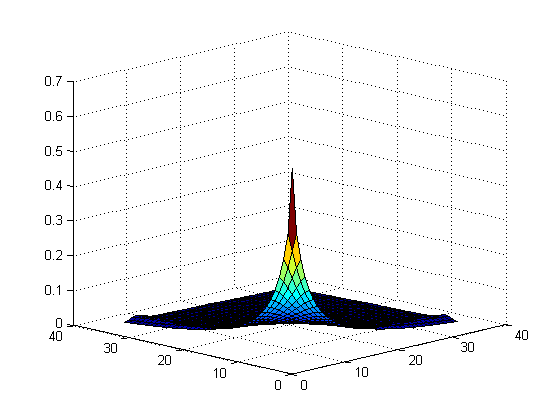
\includegraphics[width=\linewidth]{schema2}
\caption{Without(P1SA ($\bar{\mu} =0.4$ and $c=0.999999$)}
\end{minipage}
\hspace{0.5cm}
\begin{minipage}[b]{0.45\linewidth}
\centering
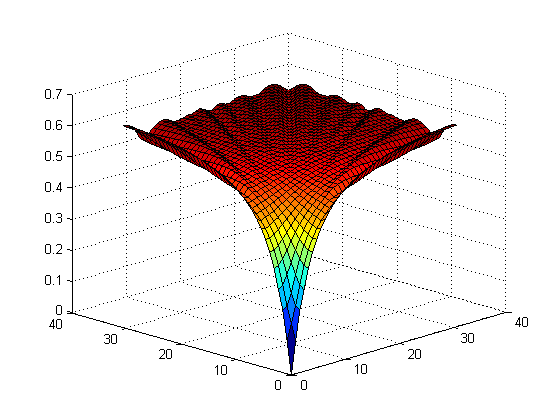
\includegraphics[width=\linewidth]{schema1}
\caption{Without ($\bar{\mu} =0.4$ and $c=0.999999$)}
\end{minipage}
\end{figure}
\end{frame}
%---------------------------------------------------------------------------------------------
\begin{frame}
\frametitle{Acceleration scheme}
2 solutions have been proposed in the past to solve this issue :
\begin{itemize}
\item Multiple sweeps : we perform $K$ sweeps without the acceleration scheme and then, 1 sweep with the acceleration scheme. 
\item Modify the update : we use the acceleration scheme for every sweep and the scalar flux is updated at every iteration, but the first moment is only updated for even iterations
\end{itemize}
\end{frame}
%---------------------------------------------------------------------------------------------
\begin{frame}
\frametitle{Acceleration scheme}
\begin{table}[H]
\begin{center}
\begin{tabular}{|c|c|c|c|c|c|}
\hline
$\bar{\mu}$ & \multicolumn{5}{c|}{spectral radius}\\
\cline{2-6}
 & 1 sweep & 2 sweeps & 4 sweeps & 8 sweeps & update\\
\hline
0 & 0.2247 & 0.3579 & 0.5119 & 0.6589 & 0.2247\\
0.2 & 0.250 &0.3822 & 0.5336 &0.6631 & 0.2506\\
0.4 & 0.6667 &0.4053 &0.5448 & 0.6703 & 0.2781\\
0.5 & 1.0 &  0.4165 &0.5580  &0.6763 &0.3536\\
0.8 & 4.0 & 0.8944 & 0.6817 & 0.7165 & 0.8944\\
0.9 & 9.0 & 1.4230 & 0.9121 & 0.8234 & 1.4230\\
0.999 & 999.0 & 15.7955 & 3.2014 & 1.6253 & 15.7955\\ 
\hline
\end{tabular}
\end{center}
\end{table}
\begin{itemize}
\item 2 sweeps scheme is less efficient than the update scheme.
\item $\rho>1$ if $\bar{\mu}=0.999$
\end{itemize}
\end{frame}
%---------------------------------------------------------------------------------------------
\begin{frame}
\frametitle{Acceleration scheme}
Fourier analysis on spatially discretized meshes. Spectral radius in function of the size of the cells in mean free path unit with $c=0.999999$ :
\begin{figure}[H]
\centering
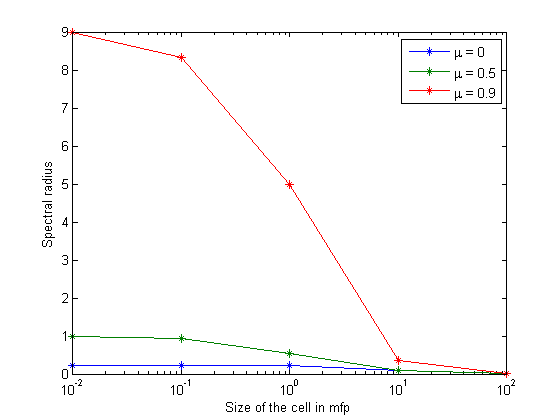
\includegraphics[width=0.7\linewidth]{DFA}
\caption{Spectral radius with discontinuous FE in function of mfp}
\end{figure}
\end{frame}
%---------------------------------------------------------------------------------------------
\begin{frame}
\frametitle{Acceleration}
When cells are very thin, we find back the results obtained without spatial discretization. However, when the size of the cells
increases, the spectral radius decreases. That is a very interesting fact since for
charged particles, $\mu \approx 1$, the mean free path is very small and the
mesh cells will likely be many mean-free-path thick. 
\end{frame}
%---------------------------------------------------------------------------------------------
\subsection{First collision source}
\begin{frame}
\frametitle{First collision source}
Penetration problem $\Rightarrow$ use a first collision source :
\begin{align}
&L \Psi = H \Phi + Q\\
&\Psi = \Psi^{inc}
\end{align}
We can write the flux as the sum of the uncollided flux and the collided flux :
\begin{align}
&L \(\Psi^u + \Psi^c\) = H \(\Phi^u + \Phi^c\) + Q\\
&\Psi^u + \Psi^c = \Psi^{inc}
\end{align}
\end{frame}
%---------------------------------------------------------------------------------------------
\begin{frame}
\frametitle{First collision source}
That we can rewrite :
\begin{align}
& L\Psi^u = 0\\
& \Psi^u = \Psi^{inc}
\end{align}
\begin{align}
& L\Psi^c = H \Phi^u + H\Phi^c + Q \label{last}\\
& \Psi^c = 0
\end{align}
If we have several groups, we can rewrite (\ref{last}) :
\begin{equation}
L \Psi^{c,g} = H \Phi^{c,g} + H \Phi ^{u,g} + \sum_{g'\neq g}H\Phi^{g'}+Q
\end{equation}
\end{frame}
%---------------------------------------------------------------------------------------------
\begin{frame}
\frametitle{First collision source}
\begin{itemize}
\item Problem: first collision source needs ray-tracing. The ``standard'' ray-tracing algorithm does not scale with the number of processors: the processor, which contains the source, has much more work than the others.
\item Solutions: dynamic load balancing, Monte-Carlo ray-tracing, others ?
\end{itemize}
\end{frame}
%---------------------------------------------------------------------------------------------
\begin{frame}
\frametitle{First collision source}
We know that the first collision source is given by (for an isotropic source) :
\begin{equation}
\begin{split}
\Phi(\br) &= \int d\br' Q(\br') \frac{e^{-\tau(\br,\br')}}{4\pi |\br - \br'|^2}\\
&\approx \sum V_i Q_i \frac{e^{-\tau (\br,\br_i)}}{4 \pi |\br - \br_i|^2}
\end{split}
\end{equation}
where $V_i$ is a volume and $Q_i$ is the source of this volume.\\
If we define :
\begin{equation}
\Delta \bo_i = \frac{A_i(\br)}{|\br - \br_i|^2}
\end{equation}
where $A_i$ is the ``visible'' surface the bloc of volume $V_i$.
\end{frame}
%---------------------------------------------------------------------------------------------
\begin{frame}
\frametitle{First collision source}
We can write :
\begin{equation}
\begin{split}
\Phi(\br) &\approx \sum_i \(\frac{Q_i}{4 \pi}\) \Delta \bo_i\ e^{-\tau(\br,\br_i)}\frac{V_i}{A_i} \\
&\approx \int_{4 \pi} d\bo \int_0^{S_{Boundary}} ds\ q(\br-s\bo) e^{-\tau (\br,\br-s\bo)}
\end{split}
\end{equation}
where $q = \frac{Q}{4\pi}$. If the source is anisotropic :
\begin{equation}
\Phi(\br) \approx \int_{4 \pi} d\bo \int_0^{S_{Boundary}} ds\ q(\br-s\bo,\bo) e^{-\tau (\br,\br-s\bo)}
\end{equation}
\end{frame}
%---------------------------------------------------------------------------------------------
\begin{frame}
\frametitle{First collision source}
So we need to know $q,\ \tau$ and $A$. We can use the convenient formulas :
\begin{align}
&\tau (\br,\br_i) = |\br-\br_i| \la \Sigma_t \ra\\
&A_{i,m} =\frac{V_i}{L_{i,m}}
\end{align}
where $L_{i,m}$ is the ``depth'' of $V_i$ in the direction $\bo_m$.\\

Now that we have the scalar flux, it is easy to compute all the moments by multiplying the scalar flux by the spherical harmonics.
\end{frame}
%---------------------------------------------------------------------------------------------
\begin{frame}
\frametitle{First collision source}
\begin{itemize}
\item We need to know $q,\ \tau$ and $A$ at the boundary of the block.
\item These quantities are not known in every points $\Rightarrow$ we will need to interpolate these quantities.
\item $\la \Sigma_t \ra$ is much smoother than $\tau$ $\Rightarrow$ we will interpolate that quantity and not $\tau$.
\item $A_i$ has to be interpolate too because the value depends on the angle through $L_{i,m}$. For the same reason, we need to interpolate $q(\br,\bo)$.
\item To be accurate enough, we need to increase the number of points where we compute these quantities at the boundary of the block. 
\end{itemize}
\end{frame}
%---------------------------------------------------------------------------------------------
\section{Optimization}
\subsection{Optimization}
\begin{frame}
\frametitle{Optimization}
\begin{itemize}
\item An important part of the radiotherapy is to optimize the rays (position
and intensity).
\item Optimization done by dividing the beams in small beamlets. Each beamlet has a constant intensity.
\item In real application, the number of beamlets is around a 1000.
\end{itemize}
\end{frame}
%---------------------------------------------------------------------------------------------
\subsection{Objective function}
\begin{frame}
\frametitle{Objective function}
The objective function is :
\begin{equation}
\min  \sum_{(i,j)\in \mathcal{T}} \(D_{ij}-\delta_{ij}\)^2 
\label{objective}
\end{equation}
$D_{ij}$ is the dose in voxel $ij$, $\delta_{ij}$ the planned dose and $\mathcal{T}$ is the tumor.
The constraints are :
\begin{equation} 
\sum_{ij \in \mathcal{D}} \nu\(D_{ij}-\delta_{ij}\)\frac{V_{ij}}{V} \leq \gamma
\label{constraint}
\end{equation}
where $V_{ij}$ is the volume of voxel $ij$, $V$ is the total volume of the organ, $\nu(x)$ is the Heaviside function and $\gamma$ is the tolerance percentage volume.\\
We also impose the dose to be positive or zero :
\begin{equation}
D_{ij} \geq 0
\label{constraint2}
\end{equation}
\end{frame}
%---------------------------------------------------------------------------------------------%
\subsection{Local minima}
\begin{frame}
\frametitle{Local minima}
\begin{itemize}
\item The objective function is convex but not the domain $\rightarrow$ several local minima.
\item Problem : 
\begin{itemize}
\item Domain : square, 5cm by 5cm.
\item Target : square in the middle of the domain, 1cm by 1cm
\item 2 beams, one from the left and one from the bottom.
\end{itemize}
\end{itemize}
\begin{figure}[H]
\centering
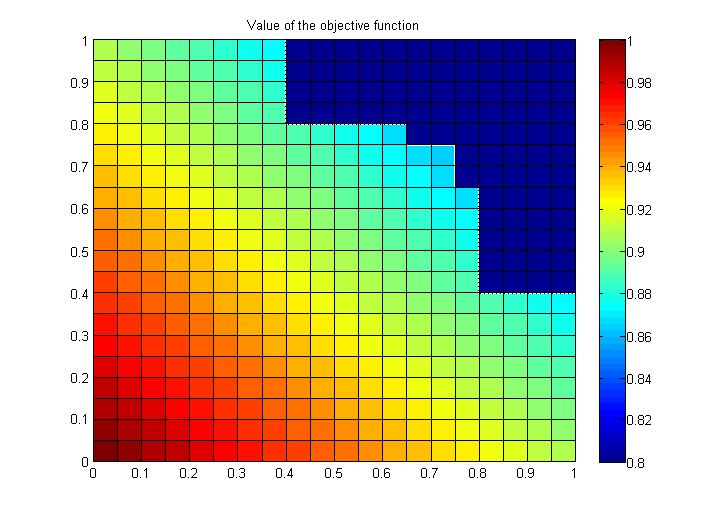
\includegraphics[width=0.45\linewidth]{dv_of_1}
\end{figure}
The area in dark blue is the forbidden area. 
\end{frame}
%---------------------------------------------------------------------------------------------%
\subsection{Methods}
\begin{frame}
\frametitle{Optimization methods}
\begin{itemize}
\item Number of local minima can be (worst case) proportional to the factorial of the number of beamlets $\Rightarrow$ deterministic method are useless.
\item Monte-Carlo methods (e.g. simulated annealing) are slow to converge because they are stochastic methods and a lot of trials have to be rejected because they are outside the domain.
\end{itemize}
\end{frame}
%---------------------------------------------------------------------------------------------%
\section{Conclusions}
\subsection{Conclusions}
\begin{frame}
\frametitle{Conclusions}
\begin{itemize}
\item Charged particles transport is challenging because of the high anisotropy of the scattering.
\item Optimization of the dose is problematic because the domain of optimization is not convex.
\end{itemize}
\end{frame}
%---------------------------------------------------------------------------------------------%
\appendix
\begin{frame}
\label{p1sa_annex}
\frametitle{P1SA Equations}
\hypertarget{p1sa_annex}{}
Putting all the terms together, we can write the scheme as :
\begin{equation}
b\left(\Phi,\boldsymbol{J},\Phi^*,\boldsymbol{J}^*\right) = l\left(\Phi^*,\boldsymbol{J}^*\right)
\label{P1SA}
\end{equation}
with :
\begin{equation}
\begin{split}
b(\Phi,\boldsymbol{J},\Phi^*,\boldsymbol{J}^*) &= \left(\Sigma_a \Phi,\Phi^*\right)_D + \left(3\Sigma_{tr} \boldsymbol{J},\boldsymbol{J}^*\right)_D+\left(\boldsymbol{\nabla} \Phi,\boldsymbol{J}^*\right)_D - \left(\boldsymbol{J},\boldsymbol{\nabla} \Phi^*\right)_D\\
&+ \frac{1}{4} \left(\llbracket\Phi\rrbracket,\llbracket\Phi^*\rrbracket\right)_{E_h^i}+\left(\llbracket\Phi\rrbracket,\ldb\boldsymbol{J}^*\rdb\cdot\boldsymbol{n}\right)_{E_h^i} -
\left(\ldb\boldsymbol{J}\cdot\boldsymbol{n}\rdb,\llbracket\Phi^*\rrbracket\right)_{E_h^i}\\
& + \frac{9}{16}\left(\llbracket \boldsymbol{J}\cdot\boldsymbol{n}\rrbracket,\llbracket \boldsymbol{J}^*\cdot\boldsymbol{n}\rrbracket\right)_{E_h^i} + \frac{9}{16}\left(\llbracket\boldsymbol{J}\rrbracket, \llbracket \boldsymbol{J}^*\rrbracket\right)_{E_h^i}\\
&+\frac{1}{4}\left(\Phi,\Phi^*\right)_{\partial D^d} + \frac{1}{2} \left(\Phi,\boldsymbol{J}\cdot \boldsymbol{n}\right)_{\partial D^d} - \frac{1}{2}\left(\boldsymbol{J}\cdot\boldsymbol{n},\Phi^*\right)_{\partial D^d}\\
&+\frac{9}{16}\left(\boldsymbol{J},\boldsymbol{J}^*\right)_{\partial D^d} + \frac{9}{16}\left(\boldsymbol{J}\cdot\boldsymbol{n},\boldsymbol{J}^*\cdot\boldsymbol{n}\right)_{\partial D^d}+\frac{9}{4} \left(\boldsymbol{J}\cdot\boldsymbol{n}, \boldsymbol{J}\cdot\boldsymbol{n}\right)_{\partial D^r}
\end{split}
\end{equation}
\end{frame}
%---------------------------------------------------------------------------------------------%
\begin{frame}
\frametitle{P1SA equations}
 and :
\begin{equation}
l(\Phi^*,\boldsymbol{J}^*) = \left(Q_0,\Phi^*\right)_D + \left(3\boldsymbol{Q}_1,\boldsymbol{J}^*\right)_D + \left(J^{inc},\Phi^*\right)_{\partial D^d} - \left(\boldsymbol{\Upsilon}^{inc},\boldsymbol{J}^*\right)_{\partial D^d}
\end{equation}
where $Q_0$ is the zeroth moment of the source, $\boldsymbol{Q}_1$ is the first moment of the source :
\begin{equation}
J^{inc} = -\sum_{\boldsymbol{\Omega}_m \cdot \boldsymbol{n}(\boldsymbol{r}_b)<0} w_m |\boldsymbol{\Omega}_m \cdot \boldsymbol{n}\left(\boldsymbol{r}_b)\right)| \Psi_m^{inc}
\end{equation}
$\Phi^d$ is the flux on the Dirichlet boundary and :
\begin{equation}
\boldsymbol{\Upsilon} = - \sum_{\boldsymbol{\Omega}_m \cdot \boldsymbol{n}(\boldsymbol{r}_b)<0} 3w_m\boldsymbol{\Omega}_m |\boldsymbol{\Omega}_m \cdot \boldsymbol{n}\left(\boldsymbol{r}_b)\right)| \Psi_m^{inc}
\end{equation}
\hyperlink{p1sa}{\beamergotobutton{back}}
\end{frame}

\end{document}



\item Problem much harder than we could expect: the objective function is
simple quadratic one but the domain is not convex $\rightarrow$ lots of local
minima.
\item Problem hard to solve even using simulated annealing ($\sim$ 500
parameters $\rightarrow$ M-C is very slow). 